\documentclass[14pt, compress, aspectratio=169]{beamer}

% can be compiled by xelatex -shell-escape presentation.tex

\usetheme[usetitleprogressbar]{m}

\usepackage[utf8]{inputenc}
\usepackage[russian, english]{babel}
\usepackage{booktabs}
\usepackage[scale=2]{ccicons}
\usepackage{listings}
\usepackage{marvosym}
\usepackage{color}
\usepackage{xcolor}
\usepackage[document]{ragged2e}
\usepackage{tikz}
\usepackage[export]{adjustbox}
\usepackage{fontawesome} 
\usepackage{enumitem}

\usetikzlibrary{shapes,arrows,positioning}
\graphicspath{{images/}}
\newfontfamily{\FA}{FontAwesome}

\definecolor{check}{rgb}{0.1,2,0.3}
\definecolor{fail}{rgb}{2,0.1,0.1}
\definecolor{question}{rgb}{0.9,0.9,0.0}

\def\twitter{{\FA \faTwitter}}
\def\github{{\FA \faGithubSign}}
\def\email{{\FA \faEnvelope}}
\def\check{\textcolor{check}{\FA \faCheck}}
\def\fail{\textcolor{fail}{\FA \faRemove}}
\def\question{\textcolor{question}{\FA \faSearch}}

\tikzstyle{block} = [rectangle, draw, fill=blue!20, text width=11em, text centered, rounded corners, minimum height=2em]
\tikzstyle{line} = [draw, -latex]

\definecolor{light-gray}{gray}{0.95}

\usepgfplotslibrary{dateplot}
\renewcommand{\ttdefault}{pcr}
\newfontfamily{\ttfamily}{Fira Code}

\lstset{
  language=SQL,
  escapeinside={(*@}{@*)},
  basicstyle=\tiny\ttfamily,
  %keywordstyle=\bfseries,
  keywordstyle=\color{blue}\ttfamily,
  backgroundcolor=\color{light-gray},
  breaklines=true,
  framexleftmargin=10pt,
  framexrightmargin=10pt,
  framextopmargin=11pt,
  framexbottommargin=10pt,
}

\title{Jsonb в PostgreSQL и NoSQL тренд}
\subtitle{сравнение функциональности и производительности}
\date{\today}
\author{Дмитрий Долгов}
\institute{}

\begin{document}

\maketitle

\section{}

\begin{frame}[fragile]
    \frametitle{Философское введение}
    NoSql популярен и это многим не дает покоя.\\
    Это приводит к тому, что многие реляционные базы данных\\
    предлагают поддержку тех или иных возможностей,\\
    изначально ассоциирующихся с NoSql.
\end{frame}
\note{
    Под NoSql в данном случае понимать документо-ориентированые и слабоструктуриванные данные, MongoDB
}

\begin{frame}[fragile]
    \frametitle{Философское введение}
    \vspace{-35pt}
    \begin{figure}
        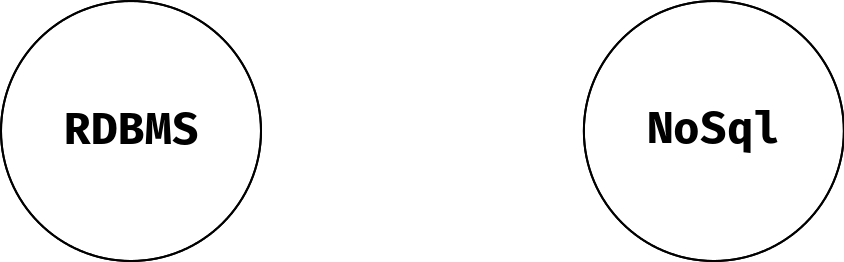
\includegraphics[width=0.8\textwidth,center]{rdbms_nosql_1.png}
    \end{figure}
\end{frame}

\begin{frame}[fragile]
    \frametitle{Философское введение}
    \vspace{-35pt}
    \begin{figure}
        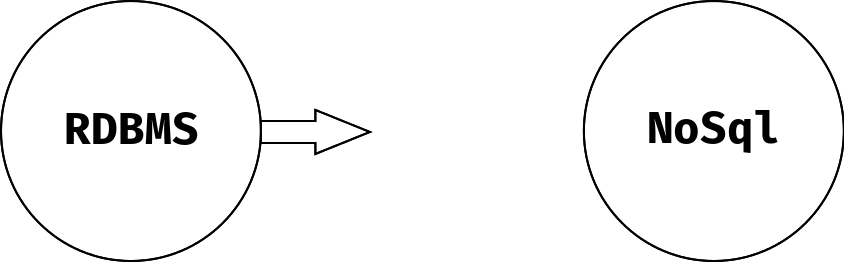
\includegraphics[width=0.8\textwidth,center]{rdbms_nosql_2.png}
    \end{figure}
\end{frame}

\begin{frame}[fragile]
    \frametitle{Философское введение}
    Почему это важно?
    Каков уровень поддержки хранения \\ слабо-структурированных данных в PostgreSQL?
\end{frame}

\begin{frame}
    \frametitle{Философское введение}
    \vspace{-35pt}
    \begin{figure}
        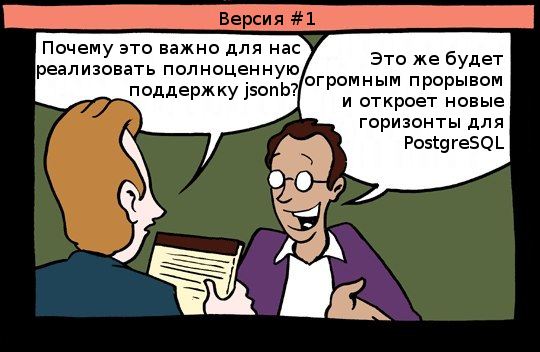
\includegraphics[width=0.8\textwidth,center]{first_option.png}
    \end{figure}
\end{frame}

\begin{frame}
    \frametitle{Философское введение}
    \vspace{-35pt}
    \begin{figure}
        
\includegraphics[width=0.8\textwidth,center]{second_option.png}
    \end{figure}
\end{frame}

\begin{frame}[fragile]
    \frametitle{Философское введение}
    \vspace{-35pt}
    \begin{figure}
        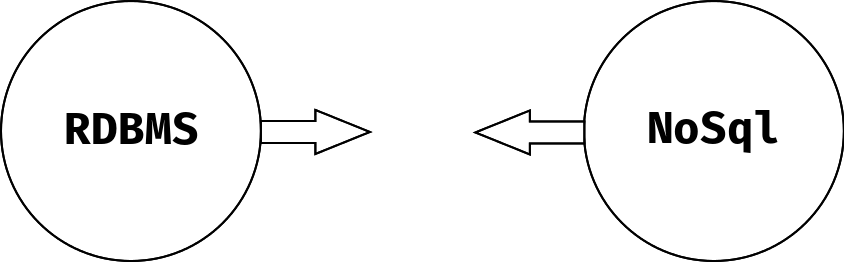
\includegraphics[width=0.8\textwidth,center]{rdbms_nosql_3.png}
    \end{figure}
\end{frame}
\note{
    Помимо PG и прочего упомянут про BI connector from MongoDB
}

\begin{frame}
    \frametitle{Философское введение}
    \vspace{-39pt}
    \begin{figure}
        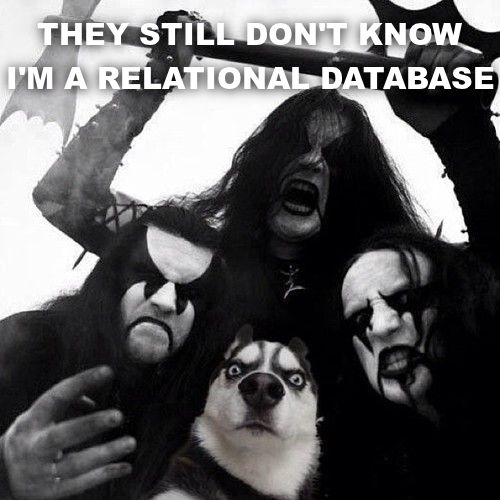
\includegraphics[width=0.55\textwidth,center]{black_metal_dog2.jpg}
    \end{figure}
\end{frame}

\section{Сравнение функционала}

\begin{frame}[fragile]
    \frametitle{Обзор по категориям}

    \begin{adjustbox}{max totalsize={1.1\textwidth}{2.0\textheight},center}
        \begin{tabular}{c | c | c | c | c | c | c | c | c | c | c}
            DB & Native & Select & Modify & Delete & Attributes & Indexing & Search & Convertion & Syntastic \\
            \hline
            PG & \check & \check & \check & \check & \check & \check & \question & \check & \question \\
            Mysql & \check & \check & \check & \check & \check & \question & \question & \fail & \question \\
            Oracle & \fail & \check & \fail & \fail & \fail & \fail & \question & \question & \question \\
            DB2 & \check & \check & \fail & \fail & \fail & \fail & \fail & \question & \fail \\
            MSSql & \fail & \check & \fail & \fail & \fail & \fail & \question & \question & \fail \\
        \end{tabular}
    \end{adjustbox}
\end{frame}

\section{PostgreSQL}

\begin{frame}[fragile]
    \frametitle{PostgreSQL}
    \begin{itemize}[label={\MVRightarrow}]
        \item Hstore
        \item Json
        \item \alert{Jsonb + (jsonbx)}
    \end{itemize}

    PostgreSQL 9.5
\end{frame}
    
\begin{frame}[fragile]
    \frametitle{Многоликий Jsonb}

  \begin{itemize}
      \item<+->
          \begin{lstlisting}[
              basicstyle=\footnotesize\ttfamily,
              showstringspaces=false,
          ]
select '"string"'::jsonb;
         
          \end{lstlisting}

      \item<+->
          \begin{lstlisting}[
              basicstyle=\footnotesize\ttfamily,
              showstringspaces=false,
          ]
select '1'::jsonb;
         
          \end{lstlisting}

      \item<+->
          \begin{lstlisting}[
              basicstyle=\footnotesize\ttfamily,
              showstringspaces=false,
          ]
select 'true'::jsonb;
         
          \end{lstlisting}

      \item<+->
          \begin{lstlisting}[
              basicstyle=\footnotesize\ttfamily,
              showstringspaces=false,
          ]
select '[1, 2, 3]'::jsonb;
         
          \end{lstlisting}

      \item<+->
          \begin{lstlisting}[
              basicstyle=\footnotesize\ttfamily,
              showstringspaces=false,
          ]
select '["string", 1]'::jsonb;
         
          \end{lstlisting}

      \item<+->
          \begin{lstlisting}[
              basicstyle=\footnotesize\ttfamily,
              showstringspaces=false,
          ]
select '{"key": {"nested": "value"}}'::jsonb;
         
          \end{lstlisting}

  \end{itemize}

\end{frame}

\begin{frame}[fragile]
  \frametitle{Получение данных}

  \begin{itemize}
      \item
          \begin{lstlisting}[
              basicstyle=\footnotesize\ttfamily,
              showstringspaces=false,
          ]
select '{"key": "value"}'::jsonb ->> 'key';
         
          \end{lstlisting}

      \item
          \begin{lstlisting}[
              basicstyle=\footnotesize\ttfamily,
              showstringspaces=false,
          ]
select '["string", (*@\alert{1}@*)]'::jsonb -> -1;
         
          \end{lstlisting}

      \item
          \begin{lstlisting}[
              basicstyle=\footnotesize\ttfamily,
              showstringspaces=false,
          ]
select '{
    (*@\alert{"key"}@*): {(*@\alert{"nested\_key"}@*): "value"}
}'::jsonb #> '{key, nested_key}'
         
          \end{lstlisting}

  \end{itemize}

\end{frame}

\begin{frame}[fragile]
  \frametitle{Изменение данных}

  \begin{lstlisting}[
      basicstyle=\footnotesize\ttfamily,
      showstringspaces=false,
  ]
select jsonb_set(
    '{"n":null, "a":{"b": 2}}'::jsonb,
    '{n}',
    '[1,2,3]'
);

            jsonb_set                                 
-------------------------------------
{"a": {"b": 2}, "n": [1, 2, 3]}
 (1 row)
 
  \end{lstlisting}

\end{frame}

\begin{frame}[fragile]
  \frametitle{Удаление данных}

  \begin{lstlisting}[
      basicstyle=\footnotesize\ttfamily,
      showstringspaces=false,
  ]

select 
    '{"a": {"b": [1, 2, (*@\alert{3}@*)]}}'::jsonb
    #-
    '{a, b, -1}';
       ?column?       
----------------------
 {"a": {"b": [1, 2]}}
(1 row)

  \end{lstlisting}
\end{frame}

\begin{frame}[fragile]
  \frametitle{Аттрибуты}

\begin{lstlisting}[
  basicstyle=\footnotesize\ttfamily,
  showstringspaces=false,
]

select jsonb_object_keys(
    '{"key": "value"}'::jsonb
);

 jsonb_object_keys 
-------------------
 key
(1 row)
         
\end{lstlisting}

\end{frame}

\begin{frame}[fragile]
  \frametitle{Аттрибуты}

\begin{lstlisting}[
  basicstyle=\footnotesize\ttfamily,
  showstringspaces=false,
]

select jsonb_typeof('1'::jsonb);

 jsonb_typeof 
--------------
 number
(1 row)

\end{lstlisting}

\end{frame}

\begin{frame}[fragile]
  \frametitle{Индексирование}

  \begin{itemize}[label={\MVRightarrow}]
    \item GIN индекс для @> <@ ?
    \item jsonb\_path\_ops
    \item jsquery: jsonb\_path\_value, jsonb\_path\_key
  \end{itemize}

\end{frame}

\begin{frame}[fragile]
  \frametitle{Поиск}

  \begin{itemize}[label={\MVRightarrow}]
    \item Содержит ли jsonb объект указанных ключ?
    \item jsquery
  \end{itemize}

\end{frame}

\begin{frame}[fragile]
  \frametitle{Конвертирование}

  \vspace{-20pt}
\begin{lstlisting}[]

select * from test_agg;
 id |   data   
----+----------
  1 | value1
  2 | value2
(2 rows)
         
\end{lstlisting}

\begin{lstlisting}[]

select jsonb_pretty(jsonb_agg(test_agg)) from test_agg;
         jsonb_pretty         
------------------------------
 [                           +
     {                       +
         "id": 1,            +
         "data": "value1"    +
     },                      +
     {                       +
         "id": 2,            +
         "data": "value2"    +
     }                       +
 ]
(1 row)

\end{lstlisting}

\end{frame}

\begin{frame}[fragile]
  \frametitle{Конвертирование}

\begin{lstlisting}[
  basicstyle=\footnotesize\ttfamily,
  showstringspaces=false,
]

select array_to_json(
    ARRAY [
        jsonb '{"a":1}',
        jsonb '{"b":[2,3]}'
    ]
);
      array_to_json       
--------------------------
 [{"a": 1},{"b": [2, 3]}]
(1 row)

\end{lstlisting}

\end{frame}

\begin{frame}[fragile]
  \frametitle{Синтаксис}

\begin{lstlisting}[
  basicstyle=\footnotesize\ttfamily,
  showstringspaces=false,
]
update some_table set jsonb_data =
    jsonb_set(jsonb_data, '{a, a1, a2}', '42');
\end{lstlisting}

vs

\begin{lstlisting}[
  basicstyle=\footnotesize\ttfamily,
  showstringspaces=false,
]

update some_table
    set jsonb_data['a']['a1']['a2'] = 42;

\end{lstlisting}

\end{frame}

\section{MySql}

\begin{frame}[fragile]
    \frametitle{MySql}

    MySql 5.7.7, тип данных JSON
\end{frame}
    
\begin{frame}[fragile]
    \frametitle{Возможные виды}

  \begin{itemize}
      \item<+->
          \begin{lstlisting}[
              basicstyle=\footnotesize\ttfamily,
              showstringspaces=false,
          ]
select cast('"string"' as json);
         
          \end{lstlisting}

      \item<+->
          \begin{lstlisting}[
              basicstyle=\footnotesize\ttfamily,
              showstringspaces=false,
          ]
select cast('["string", 1]' as json);
         
          \end{lstlisting}

      \item<+->
          \begin{lstlisting}[
              basicstyle=\footnotesize\ttfamily,
              showstringspaces=false,
          ]
select cast('{"key": {"nested": "value"}}' as json);
         
          \end{lstlisting}

  \end{itemize}

\end{frame}

\begin{frame}[fragile]
  \frametitle{Получение данных}

  \begin{itemize}
      \item
          \begin{lstlisting}[
              basicstyle=\footnotesize\ttfamily,
              showstringspaces=false,
          ]
select json_extract('{"key": "value"}', '$.*');
         
          \end{lstlisting}

      \item
          \begin{lstlisting}[
              basicstyle=\footnotesize\ttfamily,
              showstringspaces=false,
          ]
select cast('{"key": "value"}' as json) -> 'key';
         
          \end{lstlisting}

  \end{itemize}

\end{frame}

\begin{frame}[fragile]
  \frametitle{Изменение данных}

  \begin{lstlisting}[
      basicstyle=\footnotesize\ttfamily,
      showstringspaces=false,
  ]
select json_set(
    '{"n":null, "a":{"b": 2}}',
    '$.n',
    '[1,2,3]',
    '$.a',
    1
);

--------------------------
{"a": 1, "n": "[1,2,3]"}
1 row in set (0.01 sec)
 
  \end{lstlisting}

\end{frame}
\note{
    Упомянуть про то, что пока в pg нет jsonb\_insert
    для массивов
}

\begin{frame}[fragile]
  \frametitle{Удаление данных}

  \begin{lstlisting}[
      basicstyle=\footnotesize\ttfamily,
      showstringspaces=false,
  ]

select json_remove(
    '{"a": {"b": [1, 2, 3]}}',
    '$.a.b[2]'
)

----------------------
{"a": {"b": [1, 2]}}
1 row in set (0.01 sec)

  \end{lstlisting}
\end{frame}

\begin{frame}[fragile]
  \frametitle{Аттрибуты}

\begin{lstlisting}[
  basicstyle=\footnotesize\ttfamily,
  showstringspaces=false,
]

select json_type('1');

--------------
INTEGER
1 row in set (0.01 sec)

\end{lstlisting}

\end{frame}

\begin{frame}[fragile]
  \frametitle{Аттрибуты}
  Нет методов для получения ключей, значений и проч.\\
  Есть методы для получения длинны или глубины json.

\end{frame}

\begin{frame}[fragile]
  \frametitle{Индексирование}
  Тип json на прямую не индексируется, в качестве workaround\\
  предлагается создавать generated поля с json\_extract.
\end{frame}

\begin{frame}[fragile]
  \frametitle{Поиск}

  \vspace{-20pt}
  \begin{itemize}[label={\MVRightarrow}]
    \item Поиск в пути \$, *
    \item Поиск по значению json\_search
  \end{itemize}

\begin{lstlisting}[
  basicstyle=\footnotesize\ttfamily,
  showstringspaces=false,
]

select json_search(
    '{"a": "test", "b": [1, 2, "test2"]}',
    'all', 'test%'
);

--------------
["$.a", "$.b[2]"]
1 row in set (0.00 sec)

\end{lstlisting}


\end{frame}

\section{Oracle}

\begin{frame}[fragile]
    \frametitle{Oracle}

    Oracle 12.1.0.2, тип данных JSON\\
    Требует \textbf{WITH UNIQUE KEYS}
\end{frame}

\begin{frame}[fragile]
  \frametitle{Получение данных}

  \begin{itemize}
      \item
          \begin{lstlisting}[
              basicstyle=\footnotesize\ttfamily,
              showstringspaces=false,
          ]
SELECT json.document.Nested.key FROM json_data json;
         
          \end{lstlisting}

      \item
          \begin{lstlisting}[
              basicstyle=\footnotesize\ttfamily,
              showstringspaces=false,
          ]
SELECT json_value(document, '$.Number' RETURNING NUMBER) FROM json_document;

         
          \end{lstlisting}

  \end{itemize}

\end{frame}

\begin{frame}[fragile]
  \frametitle{Полнотекстовый поиск}

\vspace{-20pt}
\begin{lstlisting}[
  basicstyle=\footnotesize\ttfamily,
  showstringspaces=false,
]
CREATE INDEX json_search_idx ON json_data (document)
  INDEXTYPE IS CTXSYS.CONTEXT
  PARAMETERS (
      'section group CTXSYS.JSON_SECTION_GROUP SYNC (ON COMMIT)'
  );

SELECT document FROM json_data WHERE json_textcontains(
    document, '$.Array.Description', 'Some description'
);

\end{lstlisting}

\begin{itemize}[label={\MVRightarrow}]
    \item AL32UTF8
    \item WE8ISO8859P1
\end{itemize}

\end{frame}
\note{
    Индекс специально для JSON
}

\begin{frame}[fragile]
  \frametitle{Конвертирование}

  \vspace{-20pt}
\begin{lstlisting}[
  basicstyle=\footnotesize\ttfamily,
  showstringspaces=false,
]
SELECT * FROM json_data json,
    json_table(
        json.document, '$'
        COLUMNS (
            json_number NUMBER PATH '$.Number'
        )
    );
\end{lstlisting}

\end{frame}

\section{DB2}

\begin{frame}[fragile]
    \frametitle{DB2}

    DB2 11 for z/OS, тип данных JSON/BSON
\end{frame}

\begin{frame}[fragile]
  \frametitle{Получение данных}

  \vspace{-20pt}
\begin{lstlisting}[
  basicstyle=\footnotesize\ttfamily,
  showstringspaces=false,
]
SELECT JSON_VAL(DATA, 'PO.productName', 's:10') FROM  JSONPO;
\end{lstlisting}

\end{frame}
\note{
    's:10' - тип желаемых данных (в данном случае первые n байтов VARCHAR)
}

\begin{frame}[fragile]
  \frametitle{Конвертирование}

  \vspace{-20pt}
\begin{lstlisting}[
  basicstyle=\footnotesize\ttfamily,
  showstringspaces=false,
]
SYSTOOLS.BSON2JSON(DATA);
SYSTOOLS.JSON2BSON(DATA);
\end{lstlisting}

\end{frame}

\section{MSSql}

\begin{frame}[fragile]
    \frametitle{MSSql}

    Sql Server 2016, тип данных JSON (внутри NVARCHAR)
\end{frame}
\note{
    не бинарный тип, т.к. беспокоятся о совместимости
}
 
\begin{frame}[fragile]
  \frametitle{Получение данных}

\begin{lstlisting}[
  basicstyle=\footnotesize\ttfamily,
  showstringspaces=false,
]
SELECT JSON_VALUE(jsonInfo, '$.info.address[0].town');
\end{lstlisting}

\end{frame}

\begin{frame}[fragile]
  \frametitle{Конвертирование}

  \vspace{-20pt}
\begin{lstlisting}[
  basicstyle=\footnotesize\ttfamily,
  showstringspaces=false,
]
SELECT * FROM OPENJSON(json, N'$');

SELECT field1, field2, field3
    FROM table1
    FOR JSON PATH, ROOT("RootKey");
\end{lstlisting}

\end{frame}

\section{Производительность}

\section{Заключение}

\begin{frame}{Contacts}
    \begin{itemize}[label={}]
        \item \href{https://github.com/erthalion/jsonbx}{\github\ github.com/erthalion/jsonbx}
        \item \href{http://twitter.com/erthalion}{\twitter\ @erthalion}
        \item \email\ 9erthalion6 at gmail dot com
    \end{itemize}
\end{frame}

\plain{Questions?}

\end{document}
